\documentclass[12pt, a4, twoside]{article}
\usepackage[utf8]{inputenc}
\usepackage{graphicx}
\usepackage[margin=0.3in]{geometry}
\usepackage{wrapfig}
\usepackage[dvipsnames]{xcolor}
\usepackage{pgfplots}
% \usepackage{color}
% \graphicspath{ {image/} }

\pgfplotsset{compat=1.18}

\title{Databases}
\author{Anna Pedersem}
\date{W6, W7, W8, W9}

\pagestyle{headings}

\begin{document}

\maketitle

\section{Databases}
\begin{center}
  \begin{itemize}
    \item There are two major types of databases
    \begin{itemize}
      \item Flat file - a type of database where all the data is contained in one file. 
      \item Relational database - a databse in which data is organised in a series of relationships, or two dimensional tables, where the columns (attribues) represent data fields and the rows (tuples) represent records. Linking of data between records in different files is done by means of a foreign key. 
    \end{itemize}
    \item The database system itself is made up of: 
    \begin{itemize}
      \item A database managment system (DBMS): 'the software that builds, maintains and provides access to a database. It also provides data dictionary facilities, file protection, and security against unauthorised use
      \item A database: an organised collection of data items which can be accessed by a database managment system. The database may consist of several linked files. 
    \end{itemize}
    \item normalisation - is the process required during the development of a rational database. It requires an understanding of the structure of the relational database, the rules followed in the database design and the steps taken to normalise data. 
    \item Database tables (entities) have certain properties:
    \begin{itemize}
      \item Each entry in the table represents one data item 
      \item The table holds data types in columns, ie. in a given attribute  all items are of the same data type such as text or integer 
      \item Each column or attribue has a unique name in that table
      \item Duplicate rows are not allowed. Each row is identifable by a unique key.
      \item Rows and colums can be viewed in any sequence at any time without affecting the table contents ie. sorted or rearranged. 
    \end{itemize}
    \item The process or normalisation is used to avoid problems in the database tables such as:
    \begin{itemize}
      \item Data redundancy such as multiple repetitions of the same data 
      \item Data integrity where new data is inserted in a different form to old data or old data is only partially deleted leaving part of a record.
    \end{itemize}
  \end{itemize}

  \begin{itemize}
    \item focusing on development, anaylsis, design of a database 
    \item Open system database - is where people have access to input information. 
    \begin{itemize}
      \item eg. subscription service, creating a new account, you are putting data into the databases. E-Banking, you need to create an online database
      \item javascript, php, SQL
    \end{itemize}
    \item database - is a structured collection of data to history 
    \item purpose - to be able to process data, to anaylse, to improve the system
    \item \textbf{different types of data bases:}
    \begin{itemize}
      \item centralised - all the data is in one place. 
      \begin{itemize}
        \item Adv - access all data at once, easier to coordinate data within the database as it is all stored in 1 location. Cheaper in comparison as you only need to purchase one slightly larger storage space, eg. a server or drive which is typically cheaper than buying 2 smaller drives 
        \item Dis - if one location is compromised everything is gone, can bottleneck (too much data going in or out at once)
      \end{itemize}
      \item distrobuted - the data is distrobuted into numerous places, can be connected through a network
      \item A distrobuted database is a type of database which consists of multiple databases that are connected with each other and are spread across different physical locations. The data that is stored on varioous physical locations can thus be managed independently of other physical locations. The communication between databases at different physical locations is thus done by a computer network. 
      \begin{itemize}
        \item Adv - Can be easily expanded as data is already spread across different physical locations. The database can be easily accessed from different networks. Often more secure than a centalised database as each location will have its own security. 
        \item Dis - Adds complexity to the database due to the different storage locations which can make the database more difficult to maintain. This type of database is very costly as it is more expensive to have numerous physical locations than one larger central locations. 
      \end{itemize}
    \end{itemize}

    \item \textbf{data warehouse} - a big building filled with servers - everything is stored in one location 
    \begin{itemize}
      \item A data warehouse is a database or collection of databases that are updated 
      \item This data is stored for man years 
      \item this database can reside on one server for a company 
      \item or it ca be on several severs for that company 
      \item The overall goal of the datawarehouse is to store data over a period over time which is used in data mining $\downarrow$
    \end{itemize}
    \item \textbf{data mining}
    \begin{itemize}
      \item looking for patterns, trends on the internet. Purpose is to predict future data, used for marketing. \textbf{ethical issues} - invasion of privacy. ethically incorrect to share/sell the data. 
      \item they get around this by you agreeing to the user licence agreement 
      \item is used by buisness 
      \item they use it to find trends which can assist sales, promotions and marketing
      \item The use it to identify future planning for the company.
    \end{itemize}
    

    \item \textbf{legal issues}
    \begin{itemize}
      \item when they use data without your permission
      \item hacking 
    \end{itemize}
    \item \textbf{data mart}
    \begin{itemize}
      \item - data that has been saved in different locations, different sections of data in a buisness, a combination of these make the data warehouse
      \item A data mart is a small data warehouse usually with data for just one area 
      \item It is still a databse on a server
      \item It is queried by Data Mining software to get valuable trends in data for a company 
    \end{itemize}
    

    % \pagebreak

    \textbf{Database managment system }
    \item a software is used to create, maintain and use a databse in a clear and efficient way. 
    \item when you have just a table it is called a flat database
    \begin{itemize}
      \item all data is in 1 table, even if they are not realted to each other 
      \item column - field - data of the same types - attribute 
      \item row - record - data related to each other - entity 
    \end{itemize}
    \item tool to anaylse databases - ERD (entity relationship diagram) - because entities are related (entity = a table??)
    \item flat database - all the information in 1 table. 
    \item \textbf{Normalise} - you can normalise a database by getting rid of many - to - many relationships, one 1 - M or 1 - 1 
    \item when data is repeated (data redundancy) easy way to see that it is not normalised, if there are blank cells. When there is no primary key for an entity. When cells have not been atomised
    \item 3 levels of normalisation N1, N2, N3 (ideal) 
    \begin{center}
      \textbf{ways to normailse this database}
      \begin{center}
        %picture here
      \end{center}
      Student - \underline{ID}, Surname

      Subject - \underline{CourseID}, Name, Teacher, Room

      Report - \underline{ReportID}, Mark
    \end{center}
    \item Atomisation - making data into the simplest form it can be by breaking it up into numerous fields. 
    \begin{itemize}
      \item Address = 90 Roberts road subiaco WA 6008
      \item Street number, street name, suberb, state, postcode
    \end{itemize}
    \item Why do we normalise - prevent redundancy, update, insert, delete anaomolies. 
    \item if an anomaly happens in a database - we can have issues. 
    \begin{itemize}
      \item \textbf{Insert Anomaly}
      \begin{itemize}
        \item An insertion anomaly occurs when data cannot be inserted into a database due to other missing data
        \item most common for fields where a foreign key must not be null, but lacks the approproate data
        \item eg. A user must have a group ID as a FK however no groups have been created yet. Thus a user cannot be inserted into the database as the groupID must not be null
        \item This can result in data redundancy due to the omission of data.
        \item 
      \end{itemize}
      \item \textbf{Delete Anomaly}
      \begin{itemize}
        \item A deletion anomaly occurs when data is unintentionally lost due to the deletion of other data
        \item eg. a database row contains \textit{Username} and \textit{User Group}, John and Fred are in the user group \underline{Contributors}, if john and fred are removed from the database, our Contributors group will also disappear. This is because we havent normalised our data, meaning the only reference 
        to the Contributors user group lies within the same database row (or record). Hence removing the only two references of our user group results in the loss of data accuracy and integrity. 
        \item This also goes to show why its important for us to normalise our data and how combining unlike information can be problematic. 
      \end{itemize}
      \item \textbf{Update Anomaly}
      \begin{itemize}
        \item An update anomaly occurs when data is only partially updated in a database
        \item A database that hasnt undergone normalisation may reference the same data element in more than one location 
        \item As these locations havent been consolidated and referenced, we have to make sure each location is manually updated 
        \item this can cause problems as we then need to spend time searching for and updating each reference to the data element 
        \item An example of this is a database containing two records, Users and mailing list, john has an email address in the users record and has the same address in the mailing list record. If john decides to change his email preferences, which in turn updates the User record for John, however the system did not automatically update the mailiing list record, leaving john with 2 associated emails and thus creating inconsistencies within the database. 
      \end{itemize}
      \item \textbf{Data Redundancy}
      \begin{itemize}
        \item occurs when the same data is entered in to or more fields of a database 
        \item eg. Joe is entered in to the name field under a record called customers. Joe is also entered in to the customer field under a record called purchases. 
        Although we are referring to the 

      \end{itemize}
      \item we normailse the database to get rid of these redundnacies 
      \item \textbf{Normalise}
      \begin{itemize}
        \item We remove many - many relationships
        \item We can add entities in, group together data that is related to each other 
        \item we create an associate entity, can have any name, eg. Student/course, timetable
        \item bc it makes an association between the two other entities.
        \item associate entity always has the many entity on it and is the child entity
        \item needs a primary key
      \end{itemize}
      \item \textbf{Cardinality}
      \begin{itemize}
        \item Represents the relationships between eneities 
        \item eg. 1 -1 , 1 - M, M - 1
      \end{itemize}
      \item \textbf{attributes}
      \begin{itemize}
        \item \underline{Primary key - underlined }
        \item Foreign key - (fk)
      \end{itemize}
    \end{itemize}
    \textbf{Integrities}
    \begin{itemize}
      \item Referenial integrity
      \begin{itemize}
        \item ensures that entities are related together through primary and foriegn key 
        \item Refential integrity states that every foreign key must reference a vlaid existing value in another table
        \item this means that for every record in a normailsed database the linking element must exist in another record 
        \item both the primary and foreign keys myst be the same data type and length.
      \end{itemize}
      \item Domain integrity 
      \begin{itemize}
        \item Make sure that the data inputed into the database is correct. Uses a data dictionary to make sure that each cell in a record/field is correct. 
        \item refers to the boundaies that shape the data entered into a database 
        \item This can be as simple as placing a limit on the length of the data item and enforcing a specific data type 
        \item Domain integrity ensures organisation and validity in a database structure 
        \item Data dictionary 
        \begin{itemize}
          \item contains the different fields of an entity, each field is different in terms in data types
          \item must have the name of the field, data type, data format / size (can add a condition, eg. more than 10 and less than 250 characters, specify the format for the boolean, date/time format)
          \item ensures that the person who enters the information (especially in an open system) enters the correct data
          \item \textbf{Data types}
          \item string 
          \item integer
          \item boolean 
          \item date.time
          \item character 
          \item float.float
        \end{itemize}
        \item metadata - descipition of data 
        \item 
      \end{itemize}
      \item Entity integrity 
      \begin{itemize}
        \item Entities must have a primary key, makes sure that each entity is unquie. 
        \item ensures the validity of primary keys 
        \item the concept states that each primary key must not be NULL 
        \item it also states that each primary key must be unquie, meaning no pk value may be the same as another pk in the same record. 
      \end{itemize}
    \end{itemize}

    \textbf{ERDs}
    \begin{itemize}
      \item ID is not underlined, foreign key does not have (fk), Recommended and price
      \item 
    \end{itemize}

  \end{itemize}

  
  \item \textbf{SQL Queries}
  \item SQL - structured query language 
  \begin{itemize}
    \item SELECT - what fields you want to include (required), most common function. * represents everything. 
    \begin{itemize}
      \item SELECT DISTINCT - only list the distinct values
    \end{itemize}
    \item FROM - what databases you want to get fields from (required)
    \item WHERE - extract records that fulfill a specific condition 
    \item ORDER BY - specifies how to sort the results 
    \item GROUP BY - In SQL statement that contains aggregate functions, list fields that are not summarised in the SELECT cause
    \item HAVING - in a SQL statement that contains aggregate functions, specifices conditions that apply to fields that are summarised in the SELECT cause
    \item UPDATE - Update data in a database 
    \item DELETE - used to delete data from a database 
    \item INSERT INTO - insert new data in a database 
    \item INNER JOIN - most common type of join
    \item BETWEEN - select values within a range
    \item CREATE TABLE - create a database
  \end{itemize}
  \textit{how do you select all the records from a table named "Persons" where "lastName" is alphabetically between (and including) "Hansen" and "Pettersen"}
  \begin{verbatim}
    SELECT * FROM Persons WHERE LastName BETWEEN 'Hansen' AND 'Pettersen'
  \end{verbatim}
  \textit{How can you return all the records from a table named "Persons" sorted desending by "firstName"}
  \begin{verbatim}
    SELECT * FROM Persons ORDER BY FirstName DESC
  \end{verbatim}
\end{center}


\section{Open systems in databse interconnectivity}
\begin{itemize}
  \item Role for open systems in database 
  \item Types of SQL 
  \begin{itemize}
    \item DML (Data manipulation language) - DML enables you to work with the data that goes into the database. DML is used to isert, select, update and delete records in a database 
    dealing with the manipulation of database. Many of your SQL statments will begin with one of the following commands:
    \begin{itemize}
      \item SELECT - retrieves data from the database
      \item INSERT - Inserts new data into the database
      \begin{verbatim}
        INSERT INTO 'example'.'teachers' ('idteachers', 'TeacherFirstName',
        'TeacherTitle') VALUES ('1', 'Tom', 'Stokes', 'Mr');
      \end{verbatim}
      \item UPDATE - Updates existing data in the database, change Hansen into Nilsen in the LastName column of the persons table
      \begin{verbatim}
        UPDATE Persons SET LastName='Nilsen' WHERE LastName='Hansen';
      \end{verbatim}
      \item DELETE - Deletes existing data from the database
      \begin{verbatim}
        DELETE FROM `example`.`students` WHERE `idstudents` = 1;
      \end{verbatim}
      \item LIKE - value FirstName starts with a 
      \begin{verbatim}
        SELECT * FROM Persons WHERE FirstName LIKE 'a%';
      \end{verbatim}
    \end{itemize}
    \item DDL (Data definition language) - You may also occasionally need to create or drop a table or other database objects SQL ebables you to do this programmically using DDL. 
    \begin{itemize}
      \item CREATE DATABASE - Creates a new database 
      \item ALTER DATABASE - Modifies the database 
      \item DROP DATABASE - Drops (deletes) a database
      \item CREATE TABLE - Creates a new table 
      \begin{verbatim}
        CREATE TABLE 'example'.'teachers' (
          'teacherID' INT NOT NULL,
          'teacherFirstName' VARCHAR(45) NULL,
          'teacherLastName' VARCHAR(45) NOT NULL,
          PRIMARY KEY('teacherID));
      \end{verbatim}

      \begin{verbatim}
        CREATE TABLE `example`.`hardware` (
	        `hardwareID` INT NOT NULL,
	        `productName` VARCHAR(45) NOT NULL,
          `idPeople` INT NOT NULL,
          PRIMARY KEY(`hardwareID`),
          FOREIGN KEY(`idPeople`) REFERENCES `example`.`people` (`idPeople`) );
      \end{verbatim}
      \item ALTER TABLE - Modifies the table 
      \begin{verbatim}
        ALTER TABLE `example`.`subject` RENAME TO  `example`.`subjects`;
      \end{verbatim}
      \begin{verbatim}
        ALTER TABLE `example`.`subjects` ADD COLUMN `idteachers` 
        INT NOT NULL AFTER `SubjectName`;
      \end{verbatim}
      \item DROP TABLE - Drops (deletes) a table
      \item ADD CONSTRAINT 
      \begin{verbatim}
        
      \end{verbatim}
    \end{itemize}
  \end{itemize}


%   ALTER TABLE `example`.`subjects` 
% ADD INDEX `idteachers_idx` (`idteachers` ASC) VISIBLE;
% ;
% ALTER TABLE `example`.`subjects` 
% ADD CONSTRAINT `idteachers`
%   FOREIGN KEY (`idteachers`)
%   REFERENCES `example`.`teachers` (`idteachers`)
%   ON DELETE NO ACTION
%   ON UPDATE NO ACTION;

  \item Wild cards 
  \begin{itemize}
    \item \textbf{.} to match any single character 
    \item \textbf{[]} to match any character in the bracket \textcolor{ForestGreen}{[xyz], will match with "x","y","z"}
    \item Same can be used to match a character range seperated by \textbf{-} \textcolor{ForestGreen}{[a-z] will mtach any characters between "a", and "z"}
    \item \textbf{*} matches any number of characters preceding it 
    \item \^ match the beginning of the string 
    \item \$ match the end of value
    \item \% Select entries that contain something 
    \begin{itemize}
      \item {\begin{verbatim}
        SELECT * FROM people WHERE firstName LIKE "a%";
      \end{verbatim}}
      \item returns only the people entries who start with a
    \end{itemize}
  \end{itemize}
  \item Role for open systems in database interconnectivity and the development and management in data driven websites 
  \item \textbf{Background}
  \begin{itemize}
    \item In order to link to a website the provides a database it needs a system of connectivity 
    \item This connectivity is a special program called an Application Program Interface (API). API is a software intermediary that allows two applications to talk to each other. Each time you use an app like Facebook, you send an instant message, or check the weather you're using an API
  \end{itemize}
  \item \textbf{Database Connectivity}
  \begin{itemize}
    \item Picture 2 components here; you on the internet and a database on the computer
    \item To get to that database it needs to be made avaliable on the internet
    \item It can only be made avaliable on the internet by using a speical type of software called an API
    \item It can also be made avaliable using Open Database Connectivity (ODBC) software. ODBC is an opern standard applucation programming interface (API) for accessing a database 
    \item The API or ODBC made the connection of database to the internet happen.
  \end{itemize}
\end{itemize}

\section{Class practice questions}
\begin{center}
  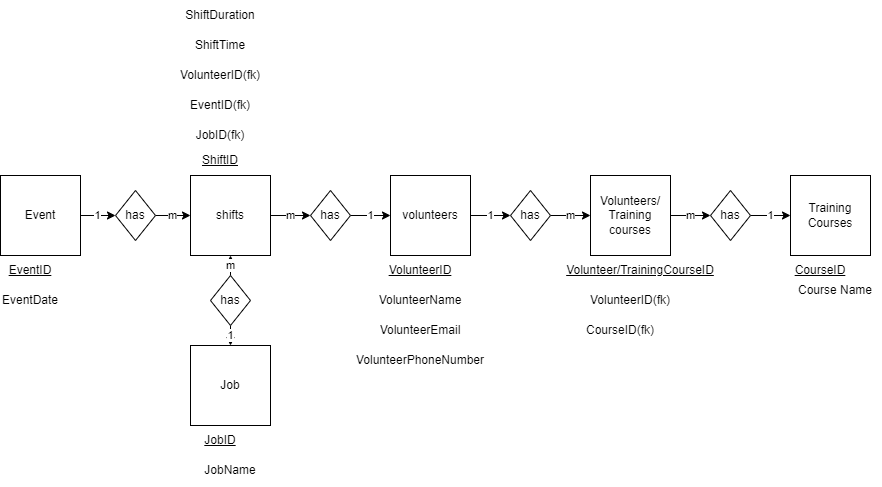
\includegraphics[width=0.8\textwidth]{ERD2.drawio}
\end{center}


\section{Practice WACE Questions}
\begin{center}
  \begin{enumerate}
    \item Data integrity is a database can be divided into 3 catagories: referential integrity, domain integrity and entity integrity
    \begin{enumerate}
      \item Outline the meaning of each of the following (\textcolor{red}{2 marks})
      \begin{itemize}
        \item Referenial integrity $\rightarrow$
        \textcolor{blue}{Referenial integrity is ensures that entities are related to each other through primary and foreign keys, it states that a foreign key must be a valid, existing value in another table}
        \item \textcolor{red}{Two entities that are related require that a foreign key musy have a matching primary key}
        \item Entity integrity $\rightarrow$
        \textcolor{blue}{Entity integrity means that each entity must have a valid primary key}
        \item \textcolor{red}{Entity integrity specificies that the primary keys on every instance of an entity must be kept, must be unique and must have values other than NULL}
      \end{itemize}
      \item Describe how data integrity can improve the process of database managment (\textcolor{red}{2 marks})
      \begin{itemize}
        % \item \textcolor{blue}{}
        \item \textcolor{red}{Data integrity is the maintence of, and the assurance of, data accuracy and consistency over its entire life-cycle and is a critical aspect to the design, implementation and usage of any system that stores, processes or retrieves data. The overall intent of any data integrity is the same: ensure data is recorded excatly as intend, such as a database correctly rejecting mutually exclusive possibilities.}
      \end{itemize}
    \end{enumerate}
  \end{enumerate}
\end{center}


\section{2021 Exam} 
\begin{center}

  \begin{itemize}
    \item 
  \end{itemize}
\end{center}

\end{document}

%information processing and technology: the HSC course @ cambridge university press 2002

% referencial integrity

%mckc0501AP!jaci
%MySQL80